\chapter{Estado del arte}
\label{chap:estado del arte}

Actualmente existen diversos tipos de herramientas que realizan tareas de recolección, filtrado y gestión de eventos dentro un sistema. Las que se han podido analizar y comprobar han sido las siguientes:

\section{Lookwise}
\hspace*{1.7in}{
\includegraphics[scale=0.5]{diagramas/lookwise-logo.png}}

Lookwise es una herramienta corporativa que hace las funciones de SIEM en materia de gestión de seguridad, Big Data y cumplimiento normativo (ISO/LOPD).

\subsection{Características}

Gestión centralizada
\begin{itemize}
\item Interfaz gráfica de administración y operación centralizada.
\item Creación y distribución de políticas de forma remota.
\item Integración de alertas y explotación de resultados.
\item Cuadro de mandos de seguridad.
\item Visibilidad en base a roles y permisos.
\item Integración con sistemas SIEM.
\end{itemize}

Comunicaciones
\begin{itemize}
\item Autenticadas y cifradas
\item Ininterrumpidas
\item Comprimidas
\end{itemize}

Plataformas soportadas
\begin{itemize}
\item Familia Windows XP (Windows Kernel 5)
\item Familia Windows 7 (Windows Kernel 6)
\end{itemize}

Arquitectura
\begin{itemize}
\item Arquitectura Distribuida.
\item Arquitectura Modular.
\item Flexible y escalable.
\item Balanceo de carga.
\item Despliegue remoto de funcionalidades y actualizaciones.
\end{itemize}
\begin{figure}[H]
\hspace*{-0.25in}{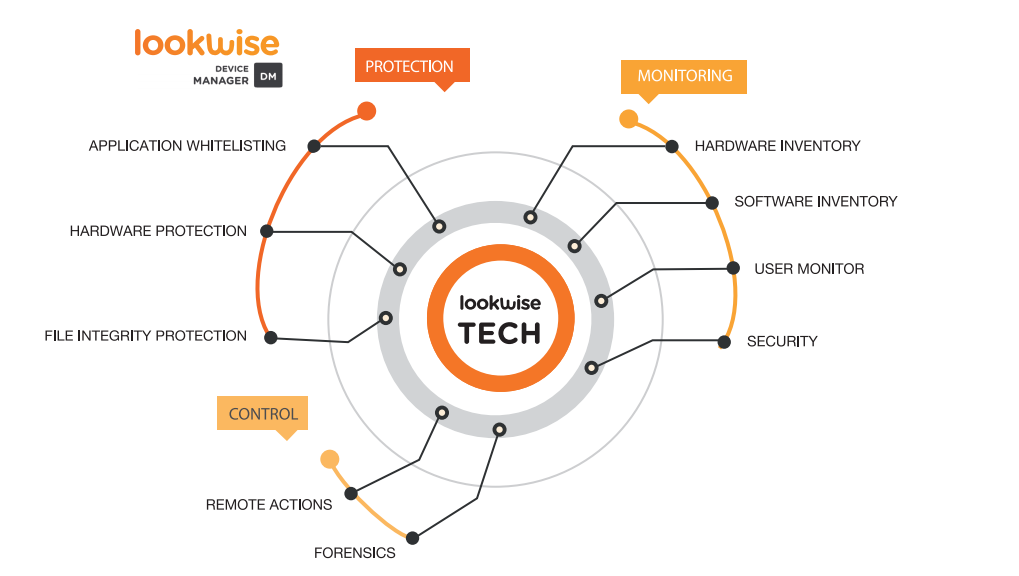
\includegraphics[scale=0.5]{diagramas/funcionalidades-lookwise.png}}
\caption{Funcionalidades Lookwise}
\end{figure}

\subsection{Análisis de la herramienta}

La herramienta de análisis de incidencias y vulnerabilidades hace la mismas funcionalidades de un SIEM pero con una capa más enfocada a sistemas PCI y de infraestructuras críticas. Gestiona eventos del sistema y los correla con alertas predefinidas internamente o que se hayan incluido cómo especificación del cliente. Detecta fallos en el Active Directory y nos genera un sistema de informe con las incidencias más graves de cara a la parte de consultoría de incidentes por parte el equipo interno.


\section{ELK Stack}

La pila ELK se basa en una solución open-source de tres productos bien diferenciados que se relacionan entre sí de la siguiente manera:

\begin{figure}[H]
\hspace*{.5in}{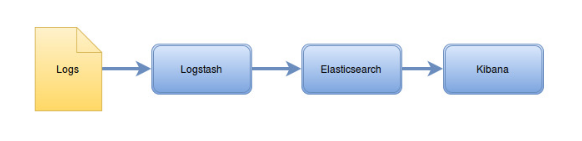
\includegraphics[scale=0.65]{diagramas/elk-stack.png}\\}
\caption{ELK Stack}
\end{figure}

\begin{itemize}
\item Elasticsearch para la búsqueda de datos y análisis en profundidad de un sistema.
\item Logstash para el registro centralizado de logs y su posterior normalización y enriquecimiento de datos.
\item Kibana cómo herramienta de visualización de los datos recolectados y procesados anteriormente según las especificaciones que queramos para el filtrado.
\end{itemize}

\subsection{Elasticsearch}
\hspace*{2in}{
\includegraphics[scale=0.15]{diagramas/elasticsearch-logo.png}\\}
Elasticsearch es un motor open-source de búsqueda y análisis de información de gran escalabilidad. Esta herramienta permite almacenar, buscar y analizar grandes volúmenes de datos de forma rápida y en tiempo real. Se suele utilizar cómo motor/tecnología subyacente de otras aplicaciones (wrapers), permitiendo así realizar funciones de búsqueda complejas de una manera más ágil.\\

\subsection{Logstash}
\begin{figure}[H]
  \hspace*{1.75in}{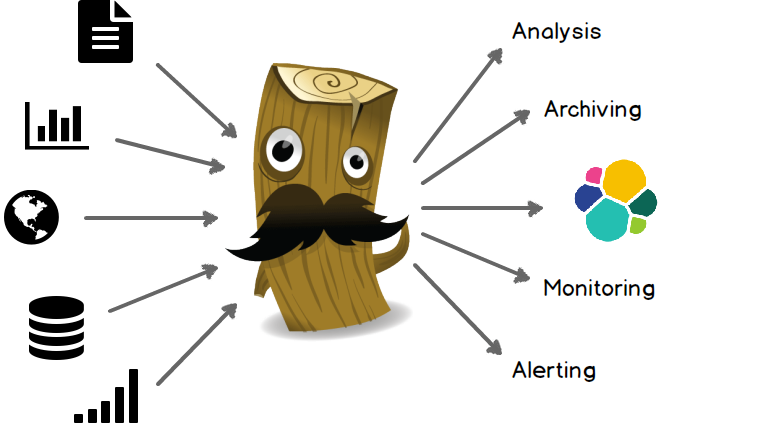
\includegraphics[scale=0.25]{diagramas/logstash.png}\\}
  \caption{Logstash description}
\end{figure}
Logstash es un motor open-source de recopilación de datos con capacidad de multihebrado en tiempo real. Esta herramienta puede unificar dinámicamente datos de diferentes fuentes y normalizar dichos datos para los outputs de nuestra elección. Además nos permite filtrar y discretizar todo los datos recolectados para obtener información analítica que pueda ser visualizada.\\

\begin{figure}[H]
  \hspace*{.5in}{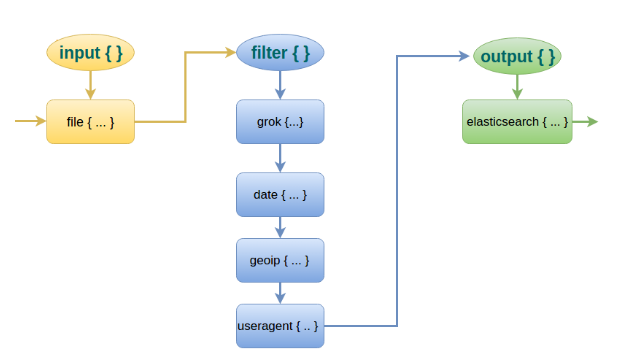
\includegraphics[scale=0.65]{diagramas/logstash-configuration.png}\\}
  \caption{Diagrama de flujo interno de logstash}
\end{figure}

Con logstash, cualquier tipo de evento puede ser enriquecido y transformado con un amplio repertorio de inputs/filtros y los datos de salida, se pueden modificar dependiendo del tipo de software sobre el que queramos introducir esos datos (plugins y códecs).\\

\subsection{Kibana}
\hspace*{2.25in}{
\includegraphics[scale=0.75]{diagramas/kibana-logo.png}\\}
Kibana es una plataforma open-source de análisis y visualización de datos diseñada para trabajar con Elasticsearch. Kibana se utiliza para para buscar, ver e interactuar con datos almacenados en los índices o base de datos de Elasticsearch. De esta forma se puede realizar fácilmente un análisis avanzado de datos que permita visualizarlo en una gran variedad de gráficas, tablas y mapas.\\

Kibana hace que sea fácil de entender y procesar grandes volúmenes de datos. Mediante su interfaz basada en un cliente web, nos permite crear de forma simple y ágil filtros sobre los datos extraidos mediante consultas a la bd de Elasticsearch en tiempo real.\\


\subsection{Análisis de la herramienta}

La pila ELK, cómo bien se ha comentado en los tres puntos anteriores nos permite recolectar, procesar y correlar cualquier tipo de logs que genere nuestro sistema de una manera visual, ágil y fácil de entender. \\

El motor de indexación de datos, Elasticsearch, nos permite obtener una ejecución en tiempo real de los logs del sistema así cómo poder escalar dicho volumen de datos dependiendo de la situación. El único inconveniente que podría sacar de este fragmento de la pila es que el sistema de referenciación de documentos internos es mediante json. Es un formato muy versátil pero incapaz de tener funcionalidad por si sola.\\

Después tenemos Logstash que es el encargado de hacer de middleware entre elastic y kibana, es decir, la parte de la recogida de muestras/eventos y la parte dónde se visualizan esas muestras. Logstash hace de filtro y de motor de normalización de datos entre los diferentes activos que tiene asignados para así poder tener todos los datos unificados según la especificación que queramos dar a cada uno de ellos. \\

Cada parte de la pila esta desarrollada en su propio lenguaje de desarrollo, siendo Java (o Groovy) el lenguaje de desarrollo de elastic, Ruby el de logstash y Javascript para Kibana. El único inconveniente que se ha podido observar es que la solución ELK está diseñada para trabajar más optimizada en entornos de cloud computing y no de manera local en un servidor. Dado que tendría que usar recursos propios de la máquina y conforme se vayan escalando nuevo recursos estos irán aumentando los de la máquina. Si hay limitación de hardware por los mismo puede llegarse a experimentar un cuello de botella entre elastic y kibana, siendo la carga de datos muy lenta y con tiempos de refresco bastante altos. \\

\section[SIEM]{Sistemas de recolección y administración de eventos: SIEM}

Un sistema de recolección y administración de eventos (SIEM), es una tecnología que se usa para la detección de amenazas y respuesta ante incidentes de seguridad a través de la obtención, en tiempo real o mediante un histórico, de eventos de seguridad a partir de una amplia variedad de fuentes o activos. Una de las principales características de un SIEM, es el gran alcance que tiene a la hora de recopilar una gran cantidad eventos para posteriormente correlar dichos eventos con alertas o incidencias de seguridad conocidas dentro del entorno corporativo.\\

\subsection{Principales características}

Estos son los puntos que principalmente gestiona un SIEM:\\

\begin{itemize}
\item Gestión de parches (actualizaciones) del kernel o software de terceros cómo adobe, java, etc.
\item Antivirus en máquinas de usuarios o en servidor.
\item Gestión de cortafuegos.
\item Integración con Active Directory (LDAP).
\item Sistema de prevención de intrusiones (en red: NIPS / basado en hosts: HIPS)
\item Proxy / Filtro de contenidos
\item Email: anti-spam / anti-phishing
\item Análisis de vulnerabilidades
\item Herramientas de seguridad opcionales:
  \begin{itemize}
  \item IPS para redes Wifi.
  \item Control de firewall web.
  \item Aplicaciones que monitoricen bases de datos.
  \item Prevención de pérdida de datos.
  \item Gestión de riesgos y herramienta de cumplimiento de políticas
  \end{itemize}
\end{itemize}

\subsection{Análisis}

Aunque esta herramienta sea cómo un conglomerado de aplicaciones o herramientas de detección y análisis, su puesta en marcha no es así tan fácil cómo cabría esperarse dado que cada despliegue requiere de unos activos o fuentes diferentes. Además, cada solución final requerirá de unas especificaciones distintas, con lo que su implantación depende en gran medida de la facilidad de adaptación al entorno y también de que los responsables de dicha herramienta tengan un profundo conocimiento sobre ella.\\

Una de las palabras más comunes que definen la implementación de un SIEM es: desalentador. A menudo termina costando más de lo previsto, requiere una experiencia sobre la herramienta que a menudo suele ser externalizada (sobre el propio fabricante) y puede llevar un tiempo considerable antes de obtener resultados tangibles.\\

Los motivos para los que generalmente se introducen un sistema cómo un SIEM en la red corporativa suelen ser varios, pero entre los más destacados suelen ser: el cumplimiento de una normativa industrial o de un gobierno, la gestión de incidentes recurrentes de seguridad o también que en la licitación de un contrato esté contemplado la puesta en marcha de este sistema para una mayor calidad del servicio prestado por un tercero o por la propia entidad. Y aún así, que la propia empresa ya gestione sus eventos internos o los monitorice, no implica que su migración al SIEM sea inmediata.\\

Además, la licitación o adquisición de un producto de estas características supone que el entorno sobre el que se va a aplicar contiene dispositivos de seguridad que monitorizar (sino se está realizando dicho control), que se dispongan de herramienta de centralización de datos (físicamente o en cloud) y que se quiera un sistema de gestión 24/7, incluido la monitorización fuera de horario laboral.\\

Son estas razones por las que a veces un sistema tan complejo y gigantesco puede que genere un sobrecoste o cubra pocas áreas de la red en las que no se tiene necesidad de vigilar. Siendo esto un incoveniente finalmente, dado que hay otras herramientas (de las que se nutre el SIEM) que ya cumplen con dicha funcionalidad a coste de tener un sistema muy pesado que gestionar.\\

--------------------------------------------------

\section{Solución tecnológica de mi proyecto}

La idea principal de mi proyecto surge fruto de la necesidad de monitorizar un red corporativa a través de un mecanismo de gestión automatizada de eventos, o lo que viene siendo un SIEM. Los pasos para la realización de este sistema se han modularizado y dividido en diferentes etapas que se acometarán cómo un todo dentro de un proyecto de investigación del grupo de ciberseguridad de la universidad de granada (UCyS - \url{http://ucys.ugr.es/}).\\

Dicho proyecto consistirá en la monitorización de la red corporativa de Mercagranada y todo lo que ello conlleva: sistemas informáticos, gestión de bases de datos, sistemas pci, sistemas perimetrales, etc. \\

[Explicar que es lo que diferencia mi pfc de las anteriores herramientas analizadas: lookwise, ELK y un SIEM. Hay otras herramientas cómo splunk o sumologic - \url{http://blog.takipi.com/log-management-tools-face-off-splunk-vs-logstash-vs-sumo-logic/}]

\section{Tecnologías implementadas}

A continuación explicaré las diferentes tecnologías/bibliotecas/lenguajes que se han empleado para la elaboración del proyecto y porque se han escogido por encima de otras posibles soluciones.

\subsection{Python}

\hspace*{1.2in}{
\includegraphics[scale=0.4]{diagramas/python-logo.png}}

Web: \url{https://www.python.org/}\\

Python es un lenguaje multiparadigma cuya estructura principal está integramente basada en objetos con sus diferentes métodos y atributos internos. Además también posee tipado dinámico, recolector/administrador de la memoria interna y un sistema de referenciado interno de atributos. \\

Las principales características que hicieron de su elección fueron:
\begin{itemize}
\item Es un lenguaje que facilita la implementación de una forma muy ágil y dinámica.
\item Su sistema de paquetes es muy intuitivo y ligero. Puedes instalar cualquier dependencia que necesites descargandola del repositorio de paquetes PyPi en el que se pueden encontrar infinidad de soluciones software dependiendo de lo que necesites. Sino, siempre se puede definir tú propio paquete software y subirlo al repositorio.
\item Es de licencia similar a la BSD (Python Software Foundation License) compatible con la GNU GPL. Así que puedes modificar cualquier aspecto del kernel del lenguaje o mejorar cualquier funcionalidad que creas oportuna.
\item Permite la fácil portabilidad entre plataformas, ya que sólo requiere de un intérprete que traduzca dicho código fuente a lenguaje máquina por lo que no existe una pesada fase de compilación por parte del sistema.
\item Tiene una amplia comunidad de desarrolladores y es muy fácil de aprender en un corto periodo de tiempo para alguien iniciado.
\item Es ampliamente usado en el mundo de la seguridad informática para ser usado en parsers, procesadores de eventos y usos con la web cómo principal reclamo (Protocolos, paquetes, tráfico, etc).
\end{itemize}


\subsubsection{Python frente a otras soluciones}

En la fase de estudio de tecnologías, se planteo la posibilidad de desarrollar el proyecto con el lenguaje de programación Java pero se descarto por los siguientes aspectos:

\begin{itemize}
\item Exige de unos conocimientos más avanzados sobre el control de procesos e hilos aunque sea más eficiente, también es más pesada la ejecución de los mismos en un sistema concurrente que puede que tenga muchos activos o fuentes que usar.
\item Lenguaje fuertemente tipado y muy estructurado.
\item Precisa de una compilación previa que pudiera incrementar los costes de empaquetar dicha solución y además solo se puede ejecutar en un entorno dónde exista una JVM o java virtual machine.
\item Para adaptar la solución obtenida a un resultado web tendría que hacer uso de un framework o IDE que ayudase a la hora de la gestión y diseño de la interfaz web así cómo la comunicación. En Python frameworks cómo Django que facilitan la tarea del despliegue en formato web y lo más cercano que se le parece es el lenguaje Groovy sobre el que se basa el software Elasticsearch.
\end{itemize}

\subsection{Procesos vs hilos}

En el proceso de desarrollo del proyecto hubo varios momentos en los que se valoró y estudio las difererencias entre un desarrollo software basado en procesos, a la hora de cada nuevo input que llegase a la monitorización, frente hilos o threads. A continuación, se hará un breve resumen sobre las diferencias entre ambos:

\subsubsection{Procesos}

Un proceso, se basa en la parte de un programa que se ejecuta en nuestro sistema, es decir, un conjunto de recursos reservados del sistema.

\subsubsection{Hilos}

Un hilo o thread, es similar a un proceso dado que hace uso de unos recursos reservados del sistema. Pero con una gran diferencia, porque si los procesos ocupan diferentes espacios de memoria, los hilos comparten ese espacio entre ellos.

\subsubsection{Problemas de los hilos}

La normal general es que un conjunto de hilos o procesos tiendan a compartir información entre ellos. Por lo que la solución de los hilos a priori parece ser la más adecuada dado que compartir información será mucho más fácil. Sin embargo, la compartición de grandes cantidades de información y haciendo un uso amplio de tareas concurrentes, pueden producir dos situaciones delicadas: el bloqueo mutuo (deadblock) y la condición de carrera (race condition).\\

\subsubsection{Hilos del kernel vs hilos del usuario}

Diferentes hilos comparten un mismo PID mientras que diferentes procesos, poseen sus propios PID. Sin embargo, esto no sucede a nivel de kernel. Los hilos del kernel tienen sus propios PID, debido a la forma en la que el kernel es ejecutado.\\

El kernel (para sistemas GNU) en sí mismo no se ejecuta cómo un proceso sino que sus tareas se ejecutan cómo parte de otros procesos. Debido a la gran cantidad de tareas que se ejecutan, en el kernel se realiza una implementación o acción alternativa para operar de forma similar a los procesos (esto es a lo que se le conoce cómo demonios).\\

\subsubsection{Solución que aplica Python}

A la hora de la implementación para comprobar que hilos se están ejecutando a través el hilo padre, se utiliza el método de la clase Thread enumerate.\\

Lo que se realiza en esa comprobación es que dentro de la pila o lista de thread que se han lanzado haya alguna coincidencia de objetos de la clase Iptables y si la hay ya existe un hilo previo en ejecución que hace las comprobaciones pertinentes.\\

\lstinputlisting{trozos-codigo/codigo-1.py}

\subsection{Django}

\hspace*{1.9in}{
\includegraphics[scale=0.15]{diagramas/django-logo.png}}

Web: \url{https://www.djangoproject.com/}\\

Django es un framework web de alto nivel para el lenguaje de programación Python. Éste framework permite un despliegue de una aplicación de escritorio al entorno web de una forma sencilla, segura y fácilmente escalable. \\

Su metodología es MVT - Model View Template en la que se explicarán en que consisten cada una de ellas:

\subsubsection{Model}

Model o Modelo es la parte encargada de la gestión con la base de datos y de abstraer su uso encapsulandola mediante clases que representan a cada una de las instancias de la BD (o tablas).\\

\subsubsection{View}

View o Vista es la parte encargada de la gestión entre la base de datos y el template. Puede llevar a confusión esta metodología de desarrollo web, ya que existe una similar: MVC. Pero en MVC (Modelo-View-Controller) el modelo se encarga de la gestión de la BD, la vista de representar los datos y el controlador de administrador o motor de contenidos entre la BD y la vista final de la aplicación web. \\

Así pues la Vista en el framework Django se representa al modelo MVC cómo el controlador.\\

\subsubsection{Template}

Template o Plantilla se refiere a la parte encargad de reprensentar la información almacenada en BD y procesada y generada mediante la Vista (View). Al contrario de un modelo MVC, en dónde el controlador se encarga de generar las vistas, en este modelo se representan las mismas cómo una plantilla de muchas otras que se van enrutando a diferentes funciones generadas por la vista. \\

Dicho esto siempre habra una plantilla Master o padre de la que heredaran todas las hijas que vayamos asociando a nuestra web. Estas heredan una estructura o skeleton en formato html enriquecido con lenguaje propio de Django en formato python. Veamos un ejemplo de plantilla Master y una plantilla que se nutre de éste skeleton:\\

\lstinputlisting[language=HTML]{trozos-codigo/codigo-2.html}

\newpage
\begin{minipage}{\linewidth}
  En el fragmento de la plantilla Master incluimos los archivos estáticos del sistema (\textbf{load staticfiles}) y además especificamos dónde iría el cuerpo de las vistas o plantillas hijas que heredarán este skeleton mediante la especificación de un bloque (\textbf{block content} y \textbf{endblock}). Y ahora veremos un ejemplo de lo que podría ir dentro de ése bloque.\\
  \lstinputlisting[language=HTML]{trozos-codigo/codigo-3.html}
  Aquí se observa perfectamente cómo se heredan las características de la plantilla Master y se define el bloque de contenido que en la plantilla Master que ya se especifico (va dentro de las etiquetas \textbf{block} y \textbf{endblock}). \\
\end{minipage}

\subsection{Dependencias Python}

Estas son las dependencias que se necesitan para la fase de desarrollo del proyecto. Para poder uso de ellas, previamente tendremos que tener instalado un entorno virtual o virtualenv desde el cual hacer la instalación de estos paquetes.

\subsubsection{Virtualenv}

Es una herramienta que nos permite crear entornos aislados de Python. De esta forma podemos realizar pruebas de dependencias o paquetes para un entorno de desarrollo, en dónde las instalaciones o pruebas no afecten a las dependencias internas del sistema.\\

\begin{itemize}
  \item Django 1.9.2: \url{https://pypi.python.org/pypi/Django/1.9.2}
  \item argparse 1.4.0: \url{https://docs.python.org/2.7/library/argparse.html}
  \item dnspython 1.12.0: \url{https://pypi.python.org/pypi/dnspython/1.12.0} - Se usa para hacer resolución directa e inversa de DNS.
  \item gunicorn 19.4.5: \url{https://pypi.python.org/pypi/gunicorn} - Sirve para desplegar un servidor WSGI (Web Server Gateway Interface) HTTP en entornos Unix.
  \item optional-django 0.3.0: \url{https://pypi.python.org/pypi/optional-django/} - Otras utilidades del framework Django
  \item pygtail 0.6.1: \url{https://pypi.python.org/pypi/pygtail} - Sirve para leer archivos de log que no se han leido aún. Similar al comando tail -f en sistemas Unix.
  \item python-dateutil 2.4.2: \url{https://pypi.python.org/pypi/python-dateutil/2.4.2} - Extensión al módulo principal de Python datetime.
  \item react 2.0.2: \url{https://pypi.python.org/pypi/react/2.0.2} - Módulo que ejecuta un servidor de datos para los componentes react de la aplicación en Python.
  \item requests 2.9.1: \url{https://pypi.python.org/pypi/requests/} - Bibloteca Python para poder consumir recursos HTTP de forma segura y controlada.
  \item setuptools 20.1.1: \url{https://pypi.python.org/pypi/setuptools} - Herramienta para la descarga, compilación, instalación, desinstalación y actualización de todos los paquetes Python. El resultado de la misma se puede usar mediante pip que se nutre el repositorio de paquetes PyPi.
  \item six 1.10.0: \url{https://pypi.python.org/pypi/six} - Es una bibloteca de compatibilidad entre Python 2 y 3.
  \item wheel 0.29.0: \url{https://pypi.python.org/pypi/wheel} - Es un gestor o generador de paquetes en Python.
  \item wsgiref 0.1.2: \url{https://pypi.python.org/pypi/wsgiref} - Es una biblioteca que sirve cómo soporte de validación para WSGI 1.0.1 para versiones de Python inferiores a la 3.2.
\end{itemize}

\subsection{C3js}

Web: \url{http://c3js.org/}\\

Es una biblioteca gráfica basada D3js, que es otra biblioteca visual en Javascript. En este caso, la biblioteca hace uso de la funcionalidad para gráficas de D3js adaptando su motor a otras posibles soluciones posibles de implementación.\\

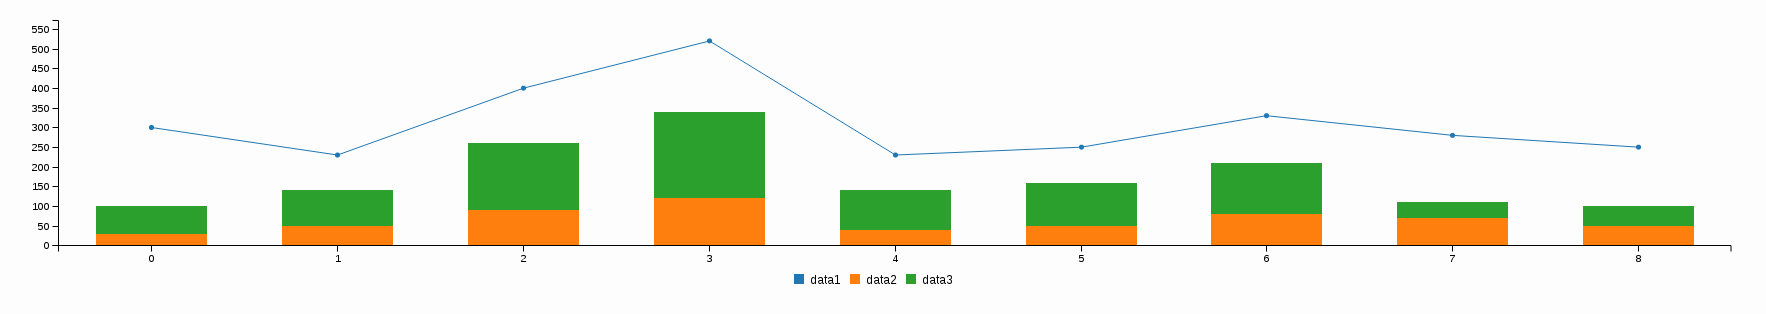
\includegraphics[scale=0.25]{diagramas/c3js-chart.png}

\subsection{D3js}
\hspace*{1in}{
\includegraphics[scale=0.35]{diagramas/d3js-logo.png}}

Web: \url{https://d3js.org/}

D3.js es una biblioteca javascript para la manipulación de documentos basado en datos. D3 nos ayuda a la hora de dar vida a los datos usando HTML, SVG y CSS de una forma sencilla y visualmente muy espectacular. Tiene su propio lenguaje que hace uso de las funcionalidades de Javascript por debajo y cuya comunidad es muy amplia en dónde podemos obtener multitud de ejemplos visuales que demuestran la capacidad de generación de gráficas y eventos de la biblioteca.\\

\begin{figure}[H]
  \hspace*{.6in}{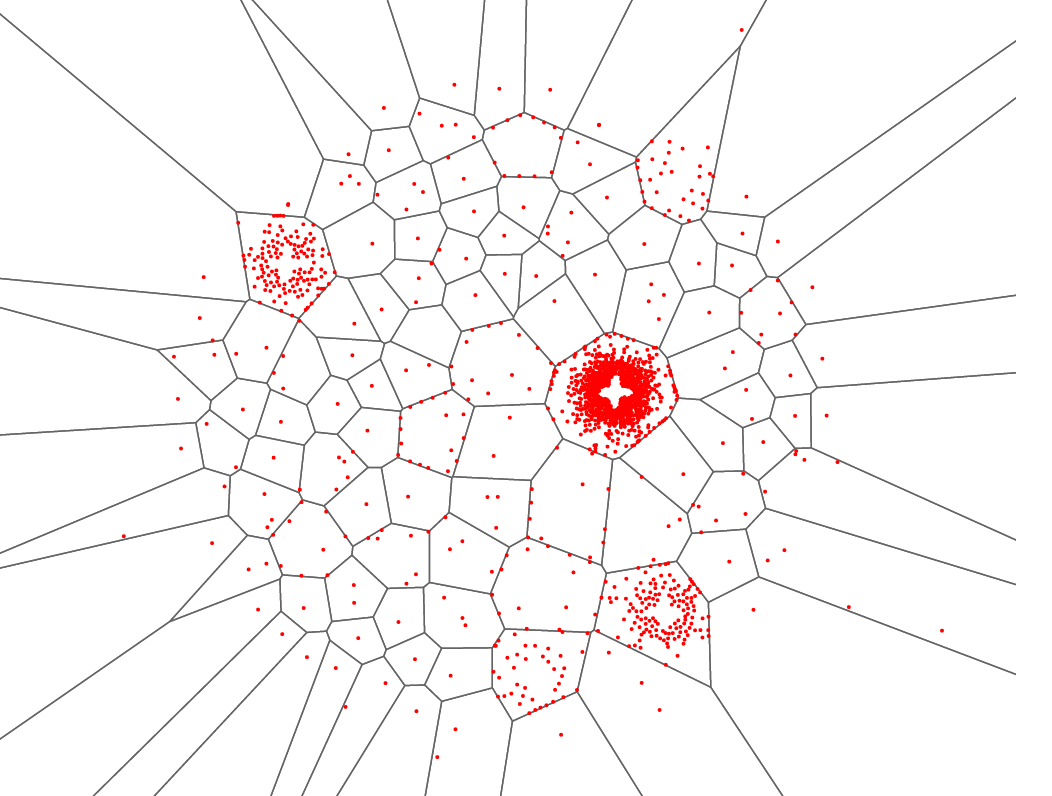
\includegraphics[scale=0.35]{diagramas/d3js-example.png}}
  \caption{Ejemplo de D3js}
\end{figure}


\subsection{\LaTeX}

Web: \url{https://www.latex-project.org/}\\

\LaTeX es un lenguaje de marcado que sirve para la redacción de documentos científicos o técnicos. Con esta herramienta o lenguaje se ha desarrollado la memoria actual del proyecto de final de carrera.

\subsection{Reactjs}

\hspace*{2.5in}{
\includegraphics[scale=0.15]{diagramas/Reactjs-logo.png}}

Web: \url{https://facebook.github.io/react/}\\

React es una biblioteca Javascript que permite construir interfaces de usuario en nuestra aplicación web. Existen soluciones similares a React cómo podría ser JQuery, pero en este caso el proceso de creación de componentes visuales se hace muy intuitiva mediante clases internas que encapsulan el contenido que posteriormente se traducirá a código Javascript nativo.\\

Para la traducción React utiliza un componente llamada JSX, pero en nuestra solución se ha usado el paquete Babel (\url{https://babeljs.io/}) que es similar pero en formato Javascript y no NodeJS.\\

\subsection{SQLite}

\hspace*{2.25in}{
\includegraphics[scale=0.5]{diagramas/sqlite-logo.png}}

Web: \url{https://www.sqlite.org/}\\

SQLite es un biblioteca software que implementa un motor para bases de datos SQL. Sus principales características son las siguientes:

\begin{itemize}
\item Las transacciones de datos son atómicas, consistentes, aisladas y durarderas (ACID) incluso después de que el sistema tengo un fallo o se apague inesperadamente.
\item No necesita de una administración o configuración previa para su normal funcionamiento.
\item Implementación de un sistema SQL integro con características más avanzadas cómo indexación parcial.
\item La base de datos, en su totalidad, se almacena cómo un archivo normal en disco. Esto es útil para ser cargado directamente cómo un archivo en una aplicación.
\item Soporta bases de datos de Terabytes de tamaño y Gigabytes de string o archivos.
\item Facilidad de uso mediante su API interna.
\item No tiene ninguna dependencia externa.
\item Multiplataforma: Android, BSD, iOS, Linux, Mac, Solaris, VxWorks y Windows soportan este tipo de formato de base de datos.
\item El código fuente está bajo dominio público para cualquier tipo de uso.
\end{itemize}

\subsection{Rsyslog}

Web: \url{http://www.rsyslog.com/}\\

Rsyslog (Rocket-Fast System for Log Processing), es un sistema de recogida de logs de sistemas UNIX (servidos mediante syslogd) que nos permite manipularlos y exportarlos a un formato más adecuado para su procesado.\\
\begin{figure}[H]
  \hspace*{.5in}{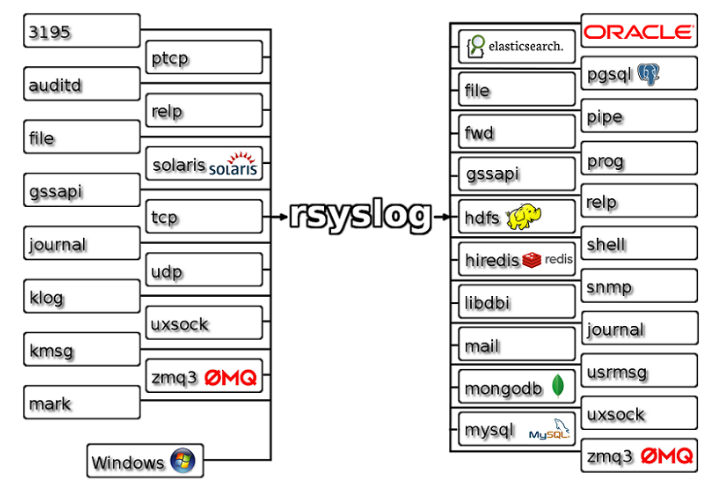
\includegraphics[scale=0.5]{diagramas/rsyslog-esquema.png}}\\
  \caption{Esquema de Rsyslog}
\end{figure}

\begin{itemize}
\item Multihilo
\item TCP, SSL, TLS RELP
\item Se puede filtrar cualquier parte de los mensajes de syslog
\item Se puede configurar el formato de salida de la recolección
\end{itemize}

\subsection{Logrotate}

Web: \url{https://github.com/logrotate/logrotate}\\
man: \url{http://linux.die.net/man/8/logrotate}\\

Es una utilidad de los sistemas UNIX que nos permite simplificar la administración de archivos de logs en un sistema en dónde haya logs de muchos tipos de fuentes. Nos permite automatizar la rotación, compresión, eliminación y envío por email de los archivos de logs del sistema. Logrotate se encuentra normalmente corriendo cómo un proceso cron diario. \\

\begin{figure}[H]
\begin{lstlisting}[language=bash]
/var/log/iptables.log
        {
                rotate 7
                daily
                missingok
                notifempty
                delaycompress
                compress
                postrotate
                        invoke-rc.d rsyslog restart > /dev/null
                endscript
        }
\end{lstlisting}
\caption{Configuración de iptables para Logrotate}
\end{figure}

Ahora se realizará una breve explicación de cada configuración que se ha establecido sobre el archivo iptables.log:

\begin{itemize}
\item \textbf{rotate <count>}: Los archivos de log son rotados una cantidad de <count> veces antes de ser eliminados o enviados por correo. Si <count> es 0, las versiones anteriores son eliminados antes de efectuarse la rotación.
\item \textbf{daily}: Los archivos de log son rotados diariamente.
\item \textbf{missingok}: Si el archivo de log no existe, ir al siguiente sin mostrar un mensaje de error.
\item \textbf{notifempty}: No rotar el log si éste está vacío.
\item \textbf{delaycompress}: Pospone la compresión de los logs previos para el siguiente ciclo de rotaciones. Esto sólo sucede cuando se combina con la opción \textbf{compress}.
\item \textbf{compress}: Las versiones antiguas de logs son comprimidas con gzip por defecto.
\item \textbf{postrotate-endscript}: Las líneas que se encuentran entre estas dos palabras en el configuración, son ejecutadas (usando /bin/sh) antes de que el archivo de log sea rotado y sólo si el log actual va a ser rotado.

  En este caso, el comando que se ejecuta fuerza a rsyslog a reabrir el archivo de log para escribir en él. Se suele usar después que logrotate mueva los archivos de logs antiguos, entonces rsyslog comienza a escribir en los nuevos.
\end{itemize}

\subsection{Syslog}

Web (man): \url{http://linux.die.net/man/3/syslog}\\

Sirve para el envío de mensajes al sistema de logs interno. syslog() genera un mensaje de log, el cuál se distribuye mediante el demonio syslogd.

\subsection{Iptables}

Web: \url{http://www.netfilter.org/projects/iptables/index.html}\\
Manual: \url{http://www.netfilter.org/documentation/HOWTO/es/packet-filtering-HOWTO-7.html}\\
man: \url{http://linux.die.net/man/8/iptables}\\

Herramienta de filtrado de paquetes IPv4/IPv6 y NAT. Iptables es usado para configurar, mantener e inspeccionar tablas de paquetes IP mediante filtros o reglas en el kernel de Linux. Se pueden definir multitud de tablas, en las que cada una pueda contener un número de reglas precargadas o que pueden ser redefinidas por el usuario. \\

\subsection{Django-rest}

\hspace*{.75in}{
\includegraphics[scale=0.5]{diagramas/django-rest-logo.png}}

Web: \url{http://www.django-rest-framework.org/}

Django REST es un framework potente y flexible que permite construir Web APIs. Se usa cómo un complemento al framework Django para el uso de API Restfull dentro de la propia aplicación.

\subsection{JSON}

Web: \url{http://www.json.org/}\\

JSON (Javascript Object Notation) es un formato de intercambio de datos ligero. Se usa para facilitar la legibilidad y escritura para los humanos y además es fácil de interpretar y parsear para una máquina. Está basado cómo un subconjunto de JavaScript y el Standard ECMA-262 3ª Edición. \\

JSON está construido sobre dos estructuras:

\begin{itemize}
\item Una colección de pares nombre/valores. En varios lenguajes, esto se realiza mediante objetos, registros, estructuras, diccionarios, tablas hash, listas de claves o arrays asociativos.
\item Una lista de valores ordenados. En la mayoría de lenguajes, esto se realiza mediante un array, un vector, lista o secuencia.
\end{itemize}

\subsection{PyCharm}

\hspace*{2.25in}{
\includegraphics[scale=0.25]{diagramas/pycharm-logo.png}}

Web: \url{https://www.jetbrains.com/pycharm/}\\

PyCharm es un IDE que permite el trabajo con aplicaciones Python en sus respectivos entornos virtuales (virtualenv) así cómo la integración con frameworks de desarrollo cómo es el caso de Django. La aplicación en sí fue desarrollada nativamente mediante un editor de texto (Emacs) pero a la hora de realizar un empaquetado e integración con otra herramientas se optó por éste IDE. \\

\subsection{Taiga}

\hspace*{2.5in}{
\includegraphics[scale=0.25]{diagramas/taiga-logo.png}}

Web: \url{https://taiga.io/}\\

Taiga es un gestor de proyectos que nos permite implementar una metodología SCRUM o Kanban sobre nuestro proyecto. Es una herramienta muy intuitiva y colaborativa, que permite definir hitos/tareas/wikis para solucionar cada punto de la fase de desarrollo de un proyecto. Además, permite la integración (WebHooks) con otras plataformas de repositorios de proyectos cómo GitHub, GitLab o BitBucket. \\
\begin{figure}[H]
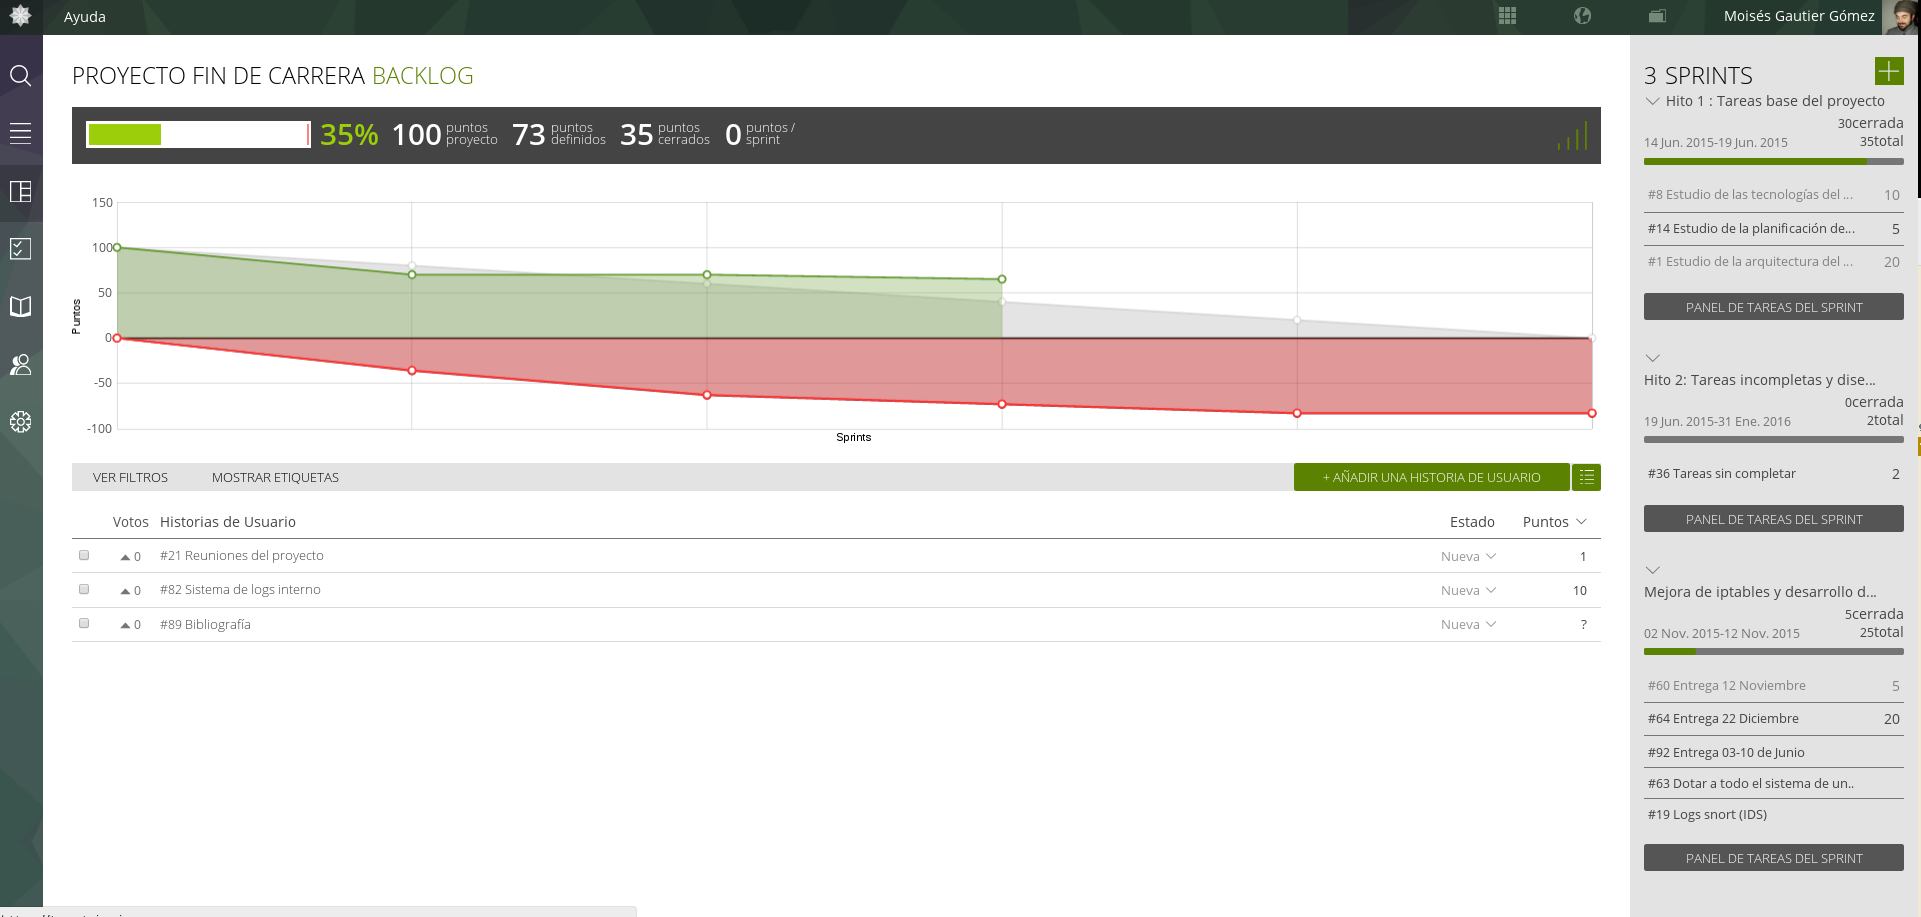
\includegraphics[scale=0.235]{diagramas/taiga-backlog.png}
\caption{Backlog del proyecto siguiendo un SCRUM}
\end{figure}

\subsection{Bitbucket}

\hspace*{2in}{
\includegraphics{diagramas/bitbucket-logo.png}}\\

Web: \url{https://bitbucket.org/}\\
Repositorio: \url{https://bitbucket.org/MGautierGomez/securityproject}\\

Gestor de repositorios Git y Mercurial. Se optó por éste gestor para probar su funcionamiento, así cómo la posibilidad de tener repositorios privados para desarrollar partes del proyecto que necesitasen ser ocultadas.\\

\subsection{Git}

\hspace*{2.1in}{
\includegraphics[scale=0.5]{diagramas/git-logo.png}}

Web: \url{https://git-scm.com/}\\

Git es un sistema open-source de control de versiones diseñado manejar integramente las fases de desarrollo de proyectos, simples y complejos, con velocidad y eficiencia.\\

\subsection{Digital Ocean}

\hspace*{1.5in}{
\includegraphics[scale=0.35]{diagramas/digital-ocean-logo.jpg}}

Web: \url{https://www.digitalocean.com/}\\

Servidor web para alojar proyectos en cloud. La ventaja de este servicio de VPS es que te permite desplegar máquinas de cualquier tipo (siempre que sean software lire) de una manera muy fácil y rápida. Además tiene un punto fuerte y es que la información se almacena en discos SSD, con lo que el procesamiento se ve muy mejorado a la hora de computar (en este caso eventos de Iptables).\\

\begin{figure}[H]
\hspace*{-.5in}{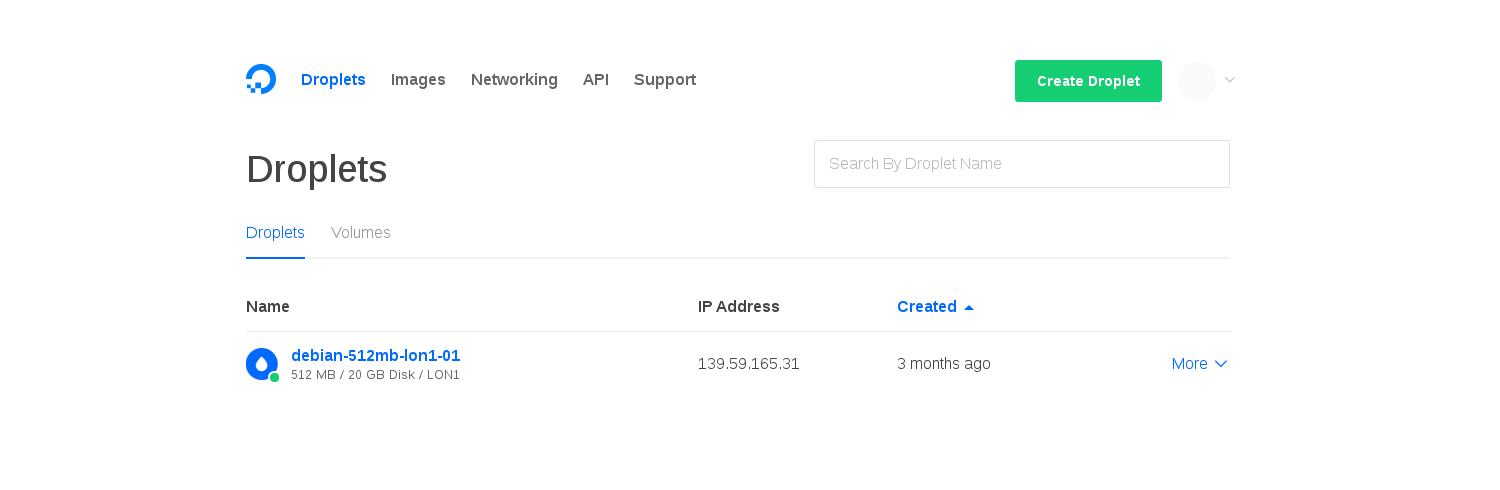
\includegraphics[scale=0.45]{diagramas/droplets.png}}
\caption{Droplet desplegado en digital ocean}
\end{figure}

\subsection{Nginx}

\hspace*{2in}{
\includegraphics[scale=0.5]{diagramas/nginx-logo.png}\\}

Web: \url{http://nginx.org/}\\
Características: \url{http://nginx.org/en/}\\

Nginx (engine x) es un servidor HTTP y proxy inverso, un servidor proxy de email y un servidor proxy genérico de TCP/UDP. Algunas de sus principales características son las siguientes:\\

\begin{itemize}
\item Sirve archivos estáticos, index y autoindexados.
\item Acelera el proceso de proxy inverso con caché: Tolerancia a fallos y carga balanceada de datos.
\item Soporta aceleración con cacheo de FastCGI, uwsgi, SCGI y servidores memcached: Tolerancia a fallos y carga balanceada de datos.
\item Soporta SSL y TLS SNI.
\item Soporta HTTP/2 con dependencia basada en prioridad y balanceo.
\end{itemize}

Configuración de nginx para el servidor en digital ocean:

\begin{figure}[H]
\begin{lstlisting}[language=bash]
server {

        root /var/www/html;

        # Tipos de archivos index de nuestro sistema

        index index.html index.htm index.nginx-debian.html;

        # Nombre del servidor en local

        server_name 139.59.165.31;

        location /static/ {
                alias ~/trunk/version-1-0/webapp/secproject/static/;
                expires 30d;
        }

        location / {
                proxy_set_header X-Forwarded-For $proxy_add_x_forwarded_for;
                proxy_set_header Host $http_host;
                proxy_redirect off;
                proxy_pass http://127.0.0.1:8000;
                proxy_pass_header Server;
                proxy_set_header X-Real-IP $remote_addr;
                proxy_connect_timeout 10;
                proxy_read_timeout 10;


        }
}
\end{lstlisting}
\caption{Configuración de nginx en digital ocean}
\end{figure}
